% Chapter: Results and Discussion (porous reframe)

\section{Solver Verification}
\label{sec:res_verification}

Before any transfer function was trusted, the solver was verified by the method of manufactured solutions and by grid and timestep convergence studies.
\reffig{fig:res_verification} summarises the canonical test cases used to validate the solver against known excitable-media phenomenology.
\reffig{fig:res_mms} shows the measured error norms against grid spacing and time step.

\begin{figure}[htbp]
\centering
\IfFileExists{../Analysis/figures/pub/pub_verification.png}{%
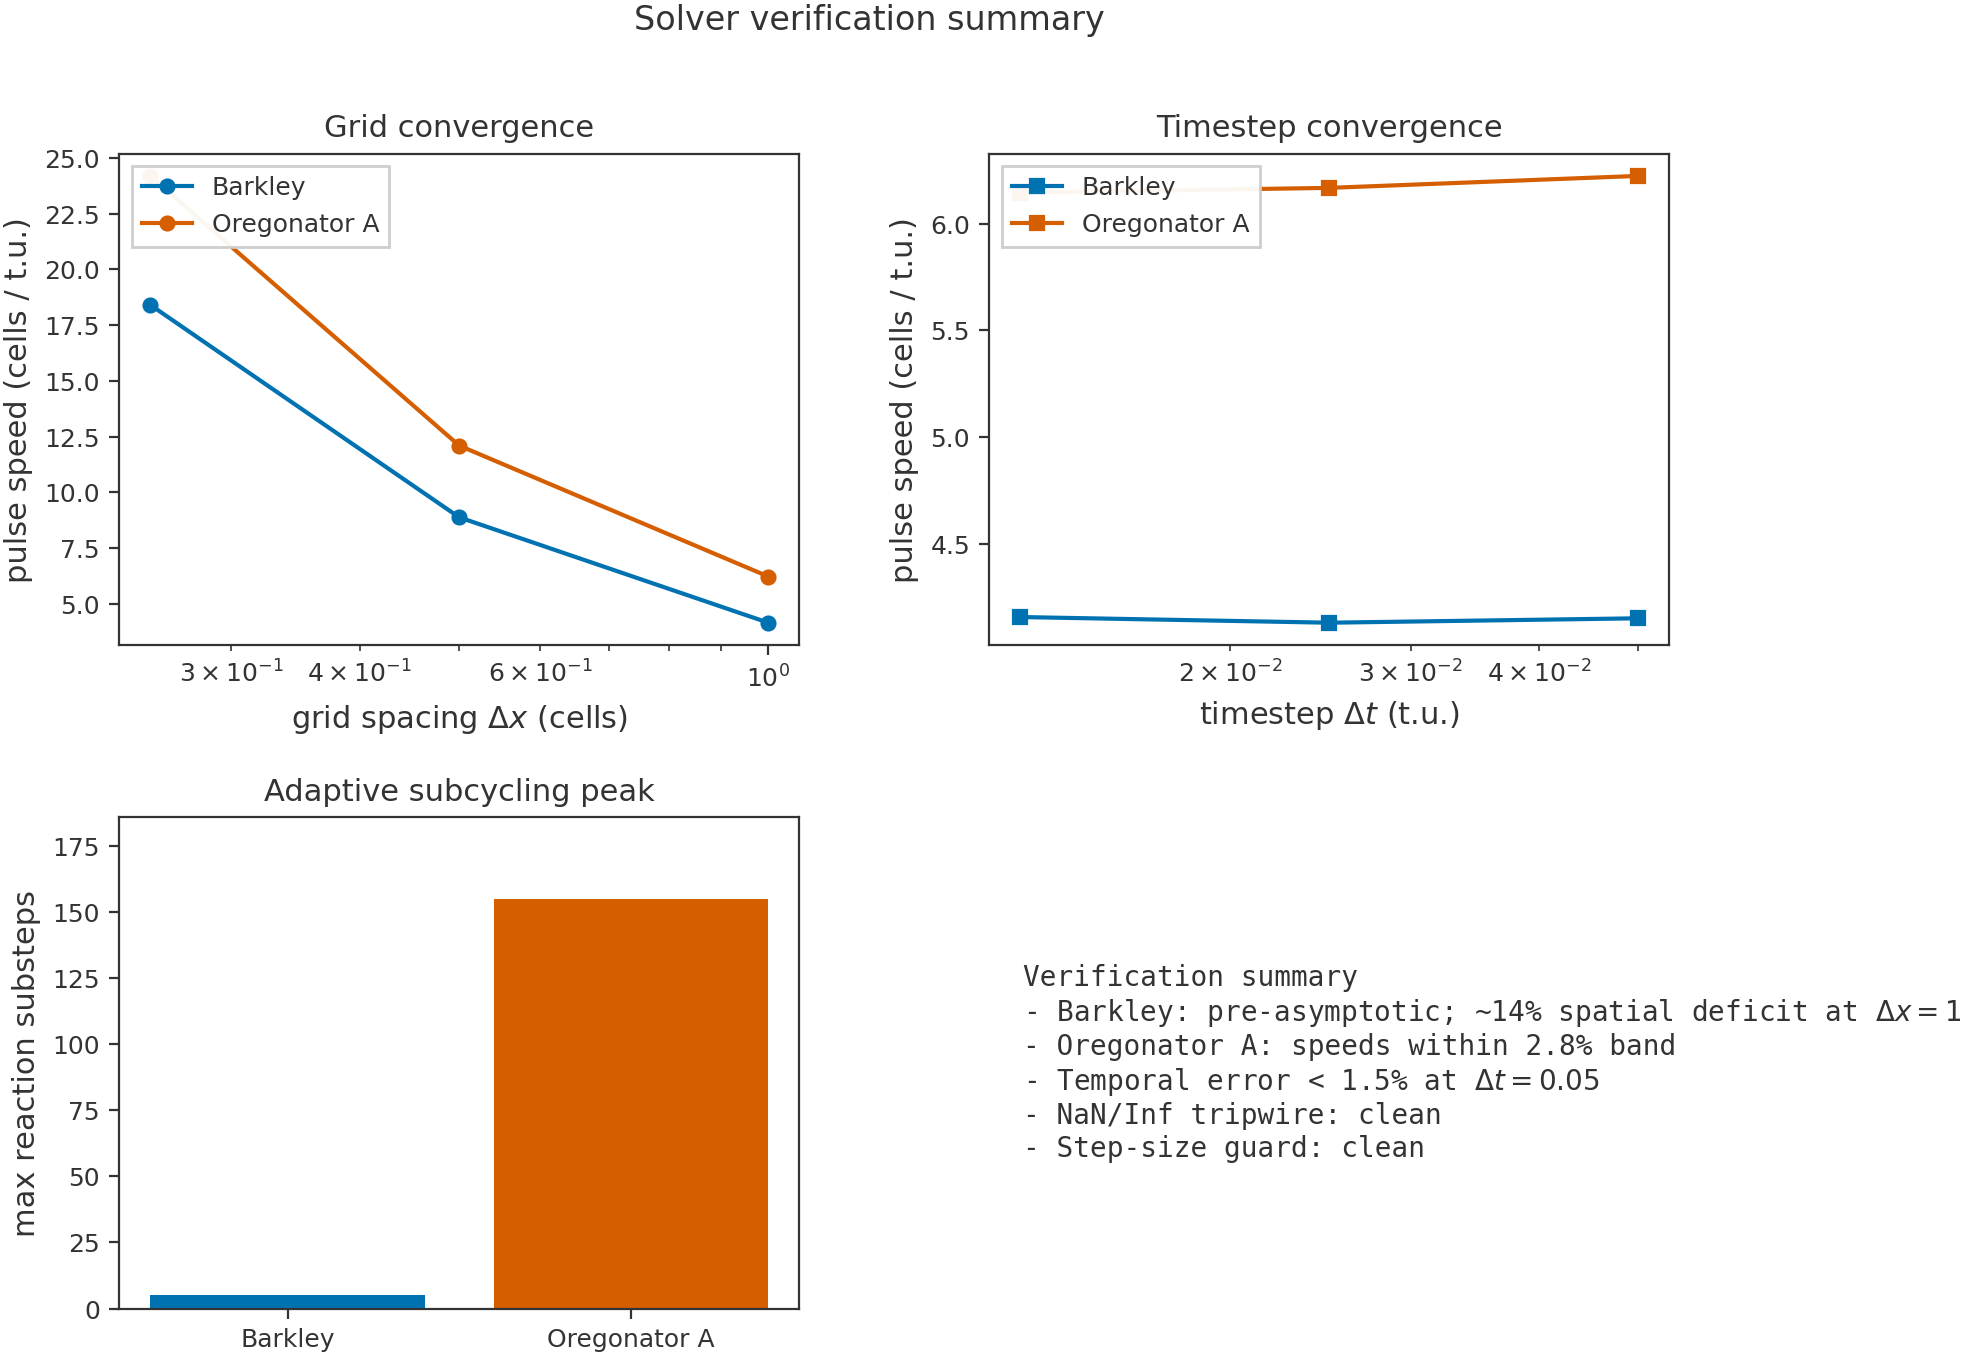
\includegraphics[width=0.95\textwidth]{../Analysis/figures/pub/pub_verification.png}}{%
[figure pending]}
\caption{Solver verification gallery: target waves, head-on collision and annihilation, gap diffraction, and timing control in the Oregonator model.}
\label{fig:res_verification}
\end{figure}
The observed spatial convergence orders at the finest refinement interval are $2.09$, $2.09$, and $1.99$ for Barkley isotropic, Barkley anisotropic, and Oregonator cases, against a design order of $2$.
The observed temporal orders are approximately $1.0$ across all cases, matching the first-order operator splitting.

Plane-pulse speed convergence is summarised in \reftab{tab:res_convergence}.
The Barkley sequence is pre-asymptotic, rising from $4.151$ cells per time unit at $\Delta x = 1$ to $4.603$ at $\Delta x = 0.25$; a Richardson extrapolation gives a continuum asymptote of approximately $4.82$, so the working resolution underestimates the Barkley speed by about $14\%$.
The Oregonator candidate-A speeds, $6.224$, $6.048$, and $6.049$, lie within a $2.8\%$ band, close to grid-converged at the working resolution.
All measurements reported below share the working resolution, so they are internally consistent as relative transfer-function measurements, and the absolute Barkley spatial deficit is stated as an explicit error bar.

\begin{figure}[htbp]
\centering
\IfFileExists{../Analysis/figures/pub/pub_mms_convergence.png}{%
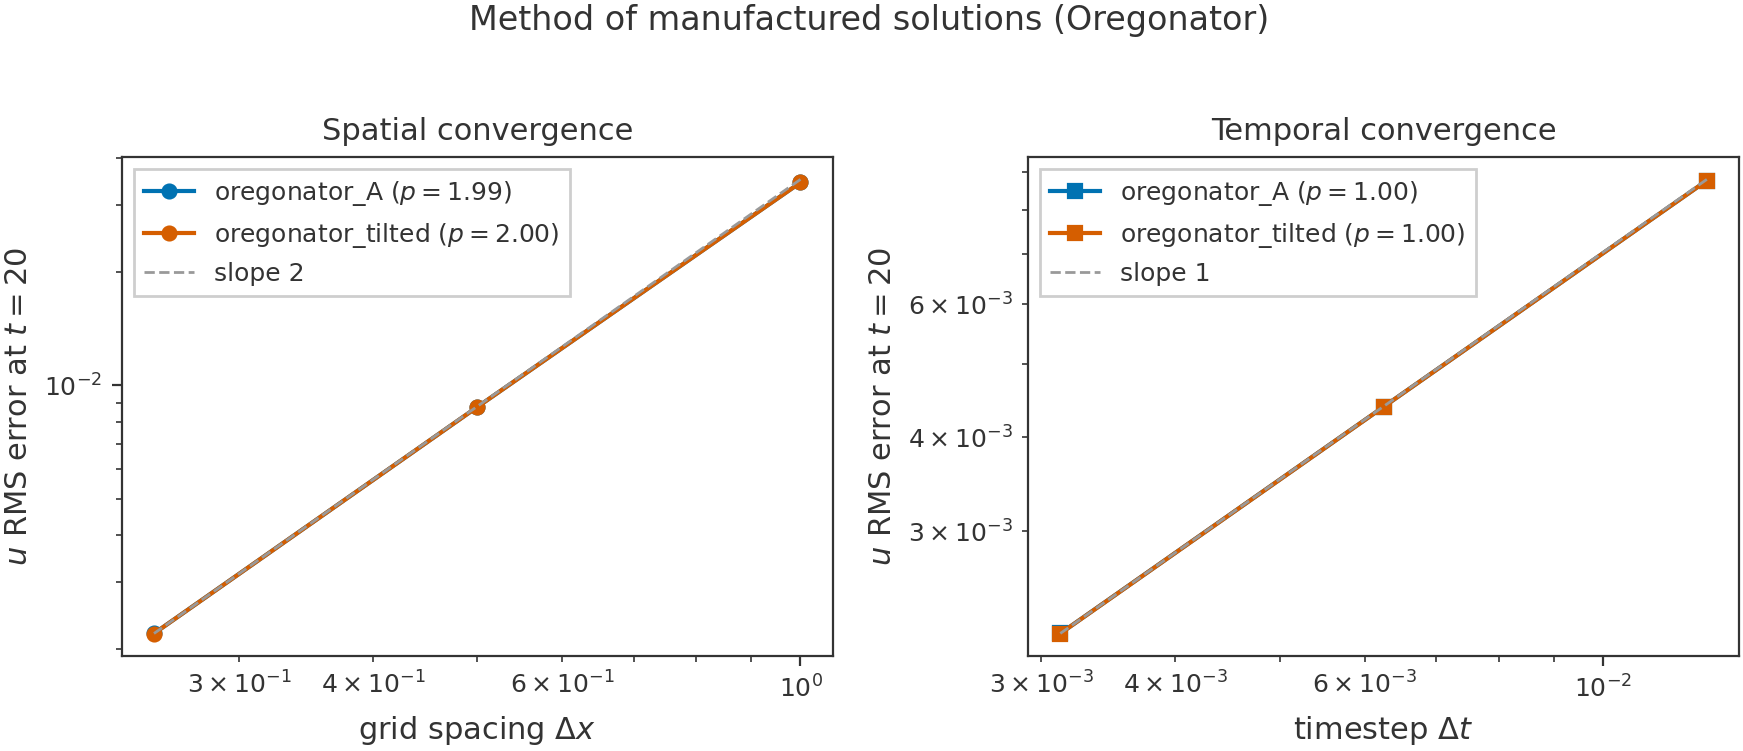
\includegraphics[width=0.9\textwidth]{../Analysis/figures/pub/pub_mms_convergence.png}}{%
[figure pending]}
\caption{Method of manufactured solutions: measured error norms against grid spacing and time step for Barkley isotropic, Barkley anisotropic, and Oregonator cases. Spatial orders are near $2$; temporal orders are near $1$.}
\label{fig:res_mms}
\end{figure}

\begin{table}[htbp]
\centering
\caption{Grid convergence of plane-pulse speed (cells per time unit) at $\Delta t = 0.05$.}
\label{tab:res_convergence}
\small
\begin{tabular}{@{}ccc@{}}
\toprule
$\Delta x$ (cells) & Barkley speed & Oregonator A speed \\
\midrule
1.00 & 4.151 & 6.224 \\
0.50 & 4.439 & 6.048 \\
0.25 & 4.603 & 6.049 \\
\midrule
Richardson asymptote & $\approx 4.82$ & n/a \\
\bottomrule
\end{tabular}
\end{table}

\section{Channel Pulse Transfer}
\label{sec:res_channel}

The wire operator was measured in a straight channel of width $W$.
A circular dark spot of radius 6 cells at the channel entrance emits a single pulse.
The free-medium dark-spot speed is $6.46$ cells per time unit and the channel speed is $6.46$--$6.47$ cells per time unit for every width from $W = 60$ down to $W = 1$.
The pulse transmits with undiminished amplitude, and no geometric wave block was observed.

The physics is that a planar front has zero curvature, so the eikonal curvature correction to its speed vanishes \cite{keener1991eikonal}.
The no-flux walls impose a zero normal derivative that a planar front already satisfies, so propagation in the channel is equivalent to a one-dimensional cable.
A straight channel is therefore a near-perfect wire whose speed and amplitude are set by the kinetics alone; width offers no computational advantage.
Structure that computes must come from junctions, curvature, or property fields.

\begin{figure}[htbp]
\centering
\IfFileExists{../Analysis/figures/pub/pub_channel_transfer_darkspot.png}{%
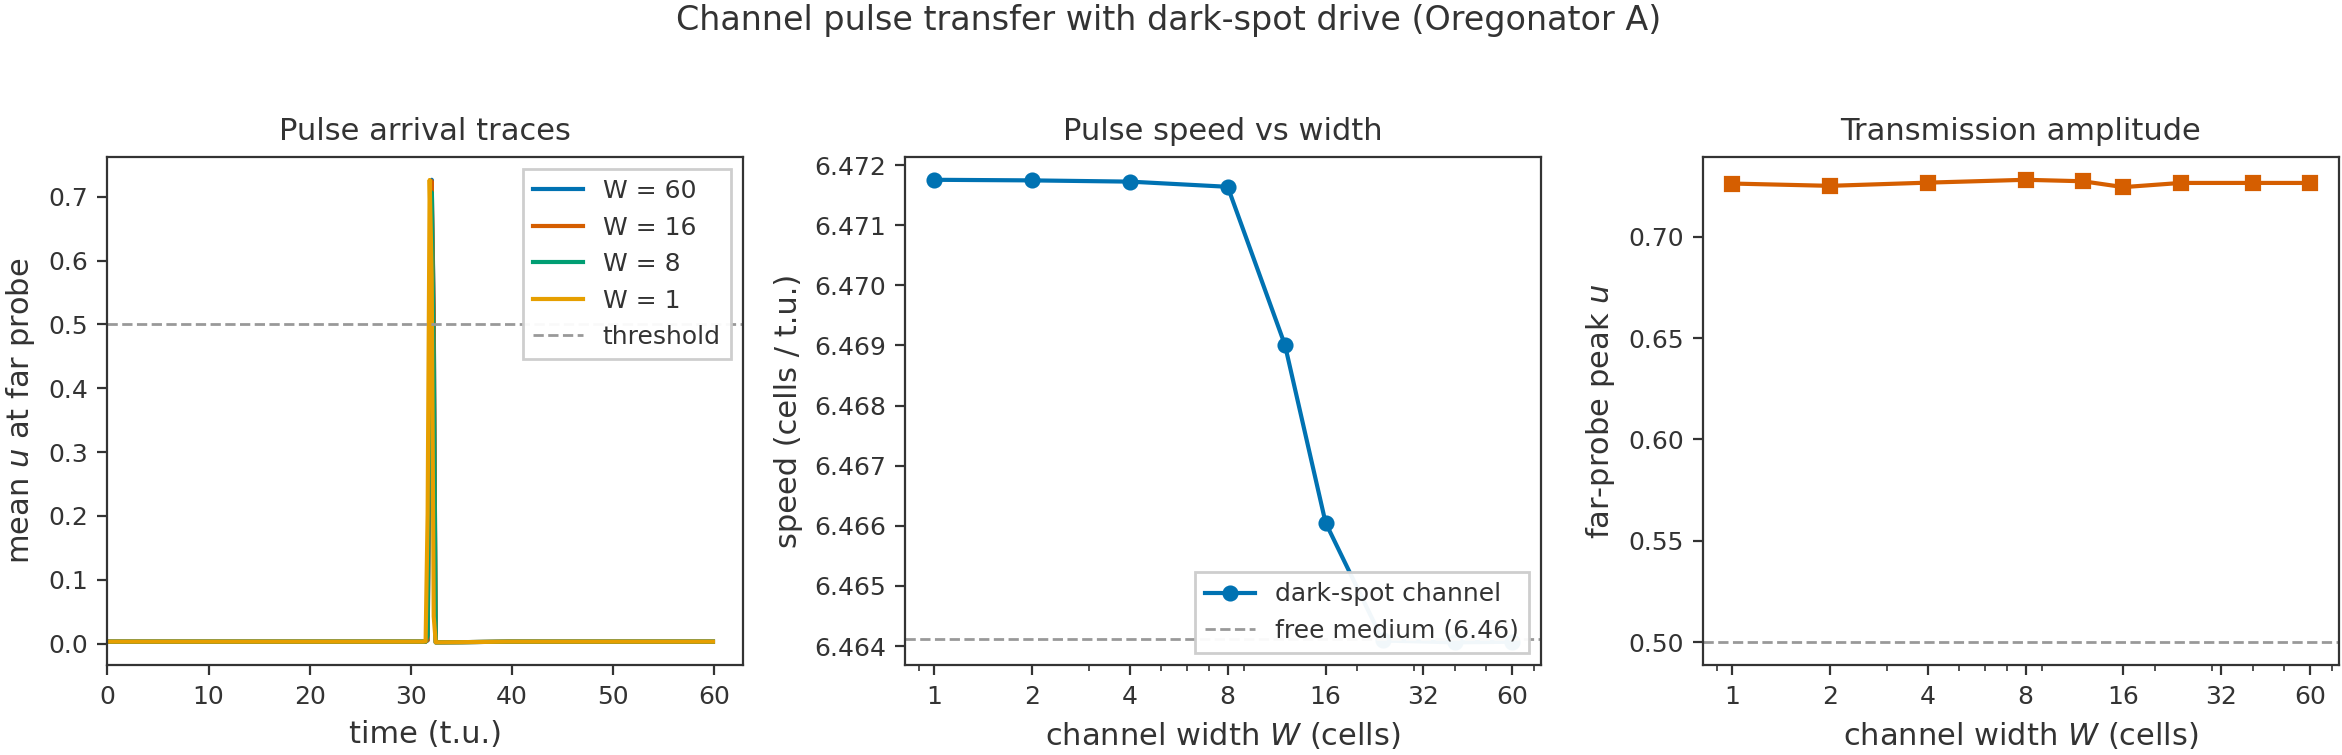
\includegraphics[width=0.9\textwidth]{../Analysis/figures/pub/pub_channel_transfer_darkspot.png}}{%
[figure pending]}
\caption{Channel pulse transfer with the dark-spot drive. A single pulse travels at the free-medium speed independent of channel width, confirming that a straight throat acts as a near-perfect wire.}
\label{fig:res_channel}
\end{figure}

\section{Frequency Response}
\label{sec:res_frequency}

The bandwidth of the wire is set by refractoriness.
The two-pulse measurement locates the absolute refractory period at $3.0$ time units for the Oregonator at candidate A.
Sustained pulse trains give the transmission curve of \reffig{fig:res_frequency}.
At low frequency the output follows the input one-to-one; the maximum 1:1 following rate is $0.167$ per time unit.
Above this rate the curve leaves unit slope and develops a staircase of dropped pulses.

The maximum 1:1 rate lies below the naive inverse of the refractory period because the dark-spot encoder itself imposes a minimum period: a flash of $3.0$ time units cannot be repeated faster than about $6.0$ time units without merging into one long pacemaker flash.
For single-event computation this constraint is irrelevant.

\begin{figure}[htbp]
\centering
\IfFileExists{../Analysis/figures/pub/pub_frequency_response_darkspot.png}{%
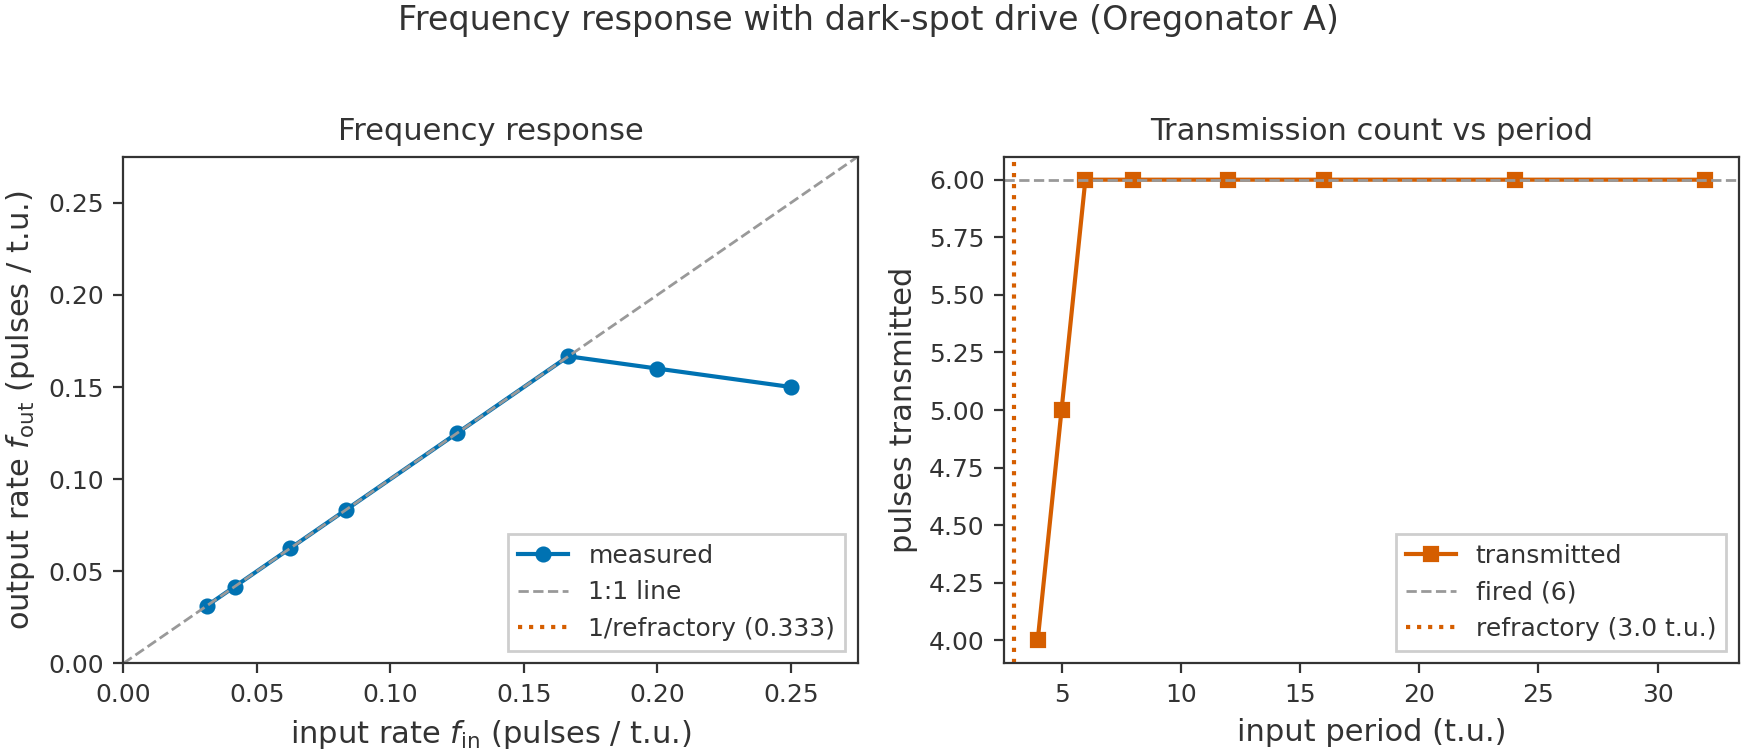
\includegraphics[width=0.85\textwidth]{../Analysis/figures/pub/pub_frequency_response_darkspot.png}}{%
[figure pending]}
\caption{Frequency response with the dark-spot drive (Oregonator A). The absolute refractory period is $3.0$ time units; the maximum 1:1 following rate is $0.167$ per time unit.}
\label{fig:res_frequency}
\end{figure}

\section{Two-Input Inhibition}
\label{sec:res_logic}

At a T-junction, the naive whole-record readout computes OR because a lone pulse diffracts into all connected branches.
With the windowed readout of \refSec{sec:meth_protocol}, the junction implements a genuine inhibition gate.
\reftab{tab:res_logic} gives the truth table for A AND (NOT B): the output probe fires when A fires alone, and is suppressed when B fires alone or when both fire.

\begin{table}[htbp]
\centering
\caption{PDE truth table for the A AND (NOT B) inhibition gate, measured in a T-junction with windowed readout.}
\label{tab:res_logic}
\small
\begin{tabular}{cccc}
\toprule
Pattern & Output peak & Output fires? \\
\midrule
00 & 0.000 & no \\
01 (B only) & 0.003 & no \\
10 (A only) & 0.706 & yes \\
11 (A+B) & 0.003 & no \\
\bottomrule
\end{tabular}
\end{table}

The separation ratio between the true output (0.706) and the strongest false output (0.003) is over $200\times$.
This inhibition operator is one of the primitives used in the graph simulator.

\begin{figure}[htbp]
\centering
\IfFileExists{../Analysis/figures/pub/pub_tjunction_logic_darkspot.png}{%
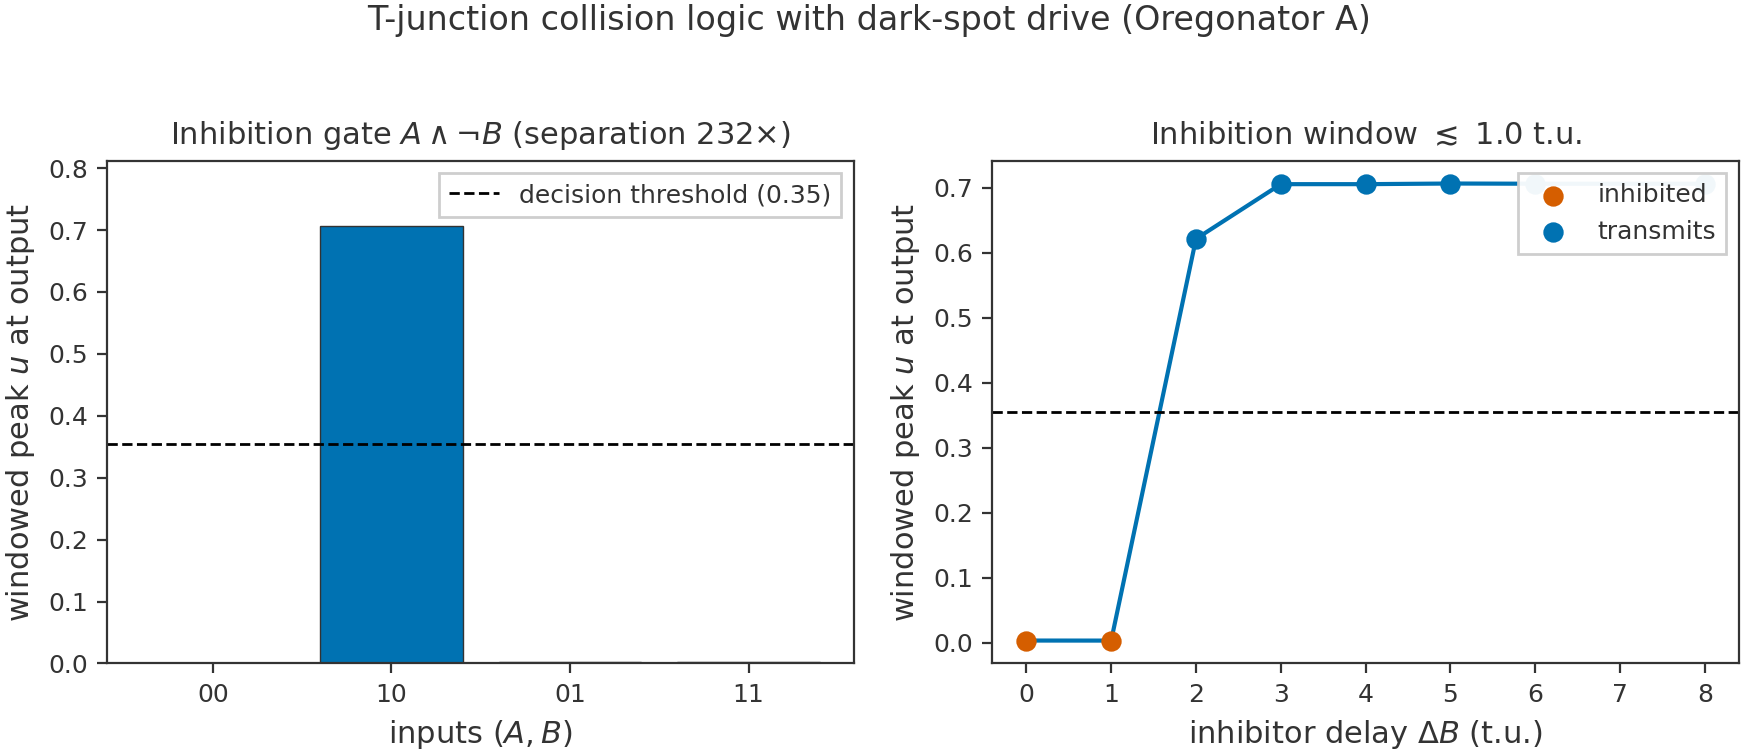
\includegraphics[width=0.9\textwidth]{../Analysis/figures/pub/pub_tjunction_logic_darkspot.png}}{%
[figure pending]}
\caption{T-junction inhibition gate with windowed readout. A alone reaches the output; B alone and A+B are suppressed, giving A AND (NOT B).}
\label{fig:res_logic}
\end{figure}

\section{Anisotropic Routing}
\label{sec:res_anisotropy}

A uniform anisotropic diffusion tensor with ratio $r = D_{\parallel}/D_{\perp}$ produces elliptical wave fronts whose fast-to-slow speed ratio is $\sqrt{r}$, confirming the eikonal prediction \cite{keener1991eikonal}.
A patch of anisotropic medium embedded in an isotropic substrate introduces direction-dependent delays.
This gives a continuous routing knob that neither walls nor light provide.

\begin{figure}[htbp]
\centering
\IfFileExists{../Analysis/figures/pub/pub_anisotropic_routing.png}{%
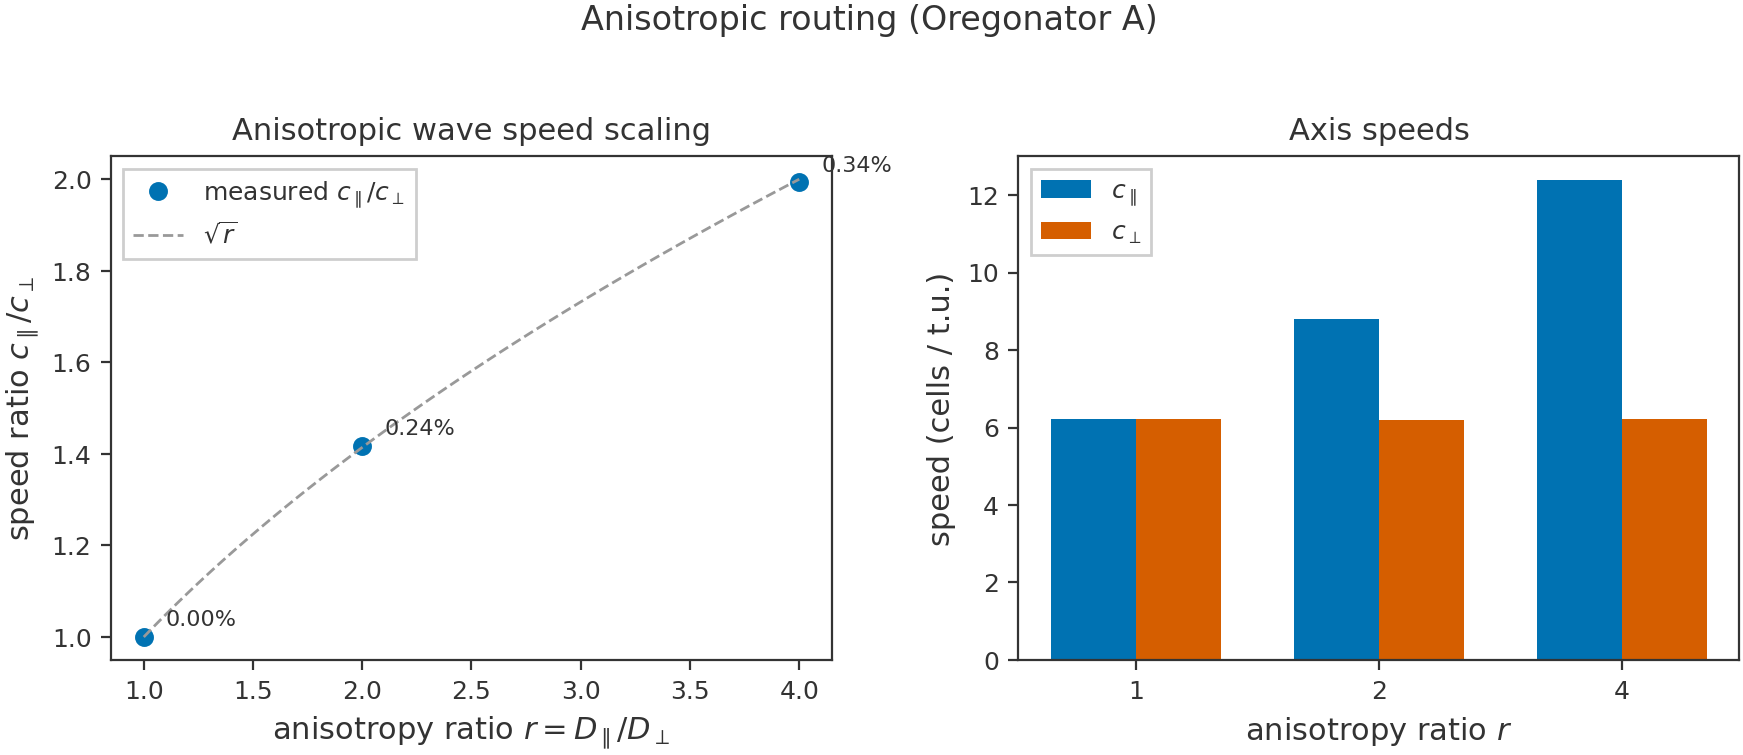
\includegraphics[width=0.9\textwidth]{../Analysis/figures/pub/pub_anisotropic_routing.png}}{%
[figure pending]}
\caption{Anisotropic routing. Elliptical wave fronts in a uniform tilted tensor field follow the eikonal $\sqrt{r}$ speed law, and an embedded anisotropic patch produces orientation-dependent delays.}
\label{fig:res_anisotropy}
\end{figure}

\section{Graph-Simulator Validation}
\label{sec:res_graph}

The measured operators were translated into the event-driven graph simulator of \refSec{sec:meth_graph}.
Three circuits were validated against full PDE solutions.

\subsection{Inhibition Gate}
\label{sec:res_graph_andnot}

The T-junction inhibition gate was modelled as a graph with nodes A, B, J, OUT and edges A$\rightarrow$J, B$\rightarrow$J, J$\rightarrow$OUT.
The routing table at J sends A to OUT and B nowhere.
\reftab{tab:res_graph_andnot} compares the graph prediction with the PDE measurement.

\begin{table}[htbp]
\centering
\caption{Graph simulator versus PDE for the A AND (NOT B) gate.}
\label{tab:res_graph_andnot}
\small
\begin{tabular}{ccccc}
\toprule
Pattern & Graph output & Graph arrival (t.u.) & PDE output peak & Match? \\
\midrule
00 & none & none & 0.000 & yes \\
01 & none & none & 0.003 & yes \\
10 & fires & 31.9 & 0.706 & yes \\
11 & none & none & 0.003 & yes \\
\bottomrule
\end{tabular}
\end{table}

The graph simulator captures the inhibition operator once the junction routing is encoded.

\subsection{Priority Router}
\label{sec:res_graph_router}

A 2-to-1 priority router was built from the same primitives: two input arms of different lengths merge into one output stem.
Arm A is shorter, so it reaches the junction first and makes it refractory; a coincident B pulse is blocked.
\reftab{tab:res_graph_router} compares graph and PDE predictions.

\begin{table}[htbp]
\centering
\caption{Graph simulator versus PDE for the 2-to-1 priority router.}
\label{tab:res_graph_router}
\small
\begin{tabular}{lccc}
\toprule
Pattern & Graph output & PDE output & Winner \\
\midrule
00 & none & none & none \\
01 (B only) & 1 pulse & 1 pulse & B \\
10 (A only) & 1 pulse & 1 pulse & A \\
11 (A+B) & 1 pulse & 1 pulse & A (shorter path) \\
\bottomrule
\end{tabular}
\end{table}

The graph simulator predicts the router before the PDE is run.

\subsection{Shared-Control Multi-Junction Gate}
\label{sec:res_graph_multi}

A shared-control gate was built in which one control input A can block two independent data paths B1 and B2.
The graph uses nodes A, B1, B2, J1, J2, O1, O2 with timing chosen so that A reaches each junction before the corresponding data pulse.
\reftab{tab:res_graph_multi} gives the graph truth table; it is correct for all eight input patterns.

\begin{table}[htbp]
\centering
\caption{Graph-simulator truth table for the shared-control gate.}
\label{tab:res_graph_multi}
\small
\begin{tabular}{ccc|cc}
\toprule
A & B1 & B2 & O1 fires? & O2 fires? \\
\midrule
0 & 0 & 0 & no & no \\
0 & 1 & 0 & yes & no \\
0 & 0 & 1 & no & yes \\
0 & 1 & 1 & yes & yes \\
1 & 0 & 0 & no & no \\
1 & 1 & 0 & no & no \\
1 & 0 & 1 & no & no \\
1 & 1 & 1 & no & no \\
\bottomrule
\end{tabular}
\end{table}

The PDE validation shows clean A-blocking for individual data pulses: O1 separation is $182\times$ and O2 separation is $192\times$.
However, pattern $011$ (both data pulses active, control absent) fails because B1 reaches J1 first, enters the shared horizontal control channel, and blocks J2 before B2 arrives.
This is a network-level crosstalk not captured by single-junction primitives.
It shows that the graph simulator must be calibrated per junction shape and that shared channels can introduce unmodelled coupling.

\begin{figure}[htbp]
\centering
\IfFileExists{../Analysis/figures/rd_multi_gate_pde_snapshots.png}{%
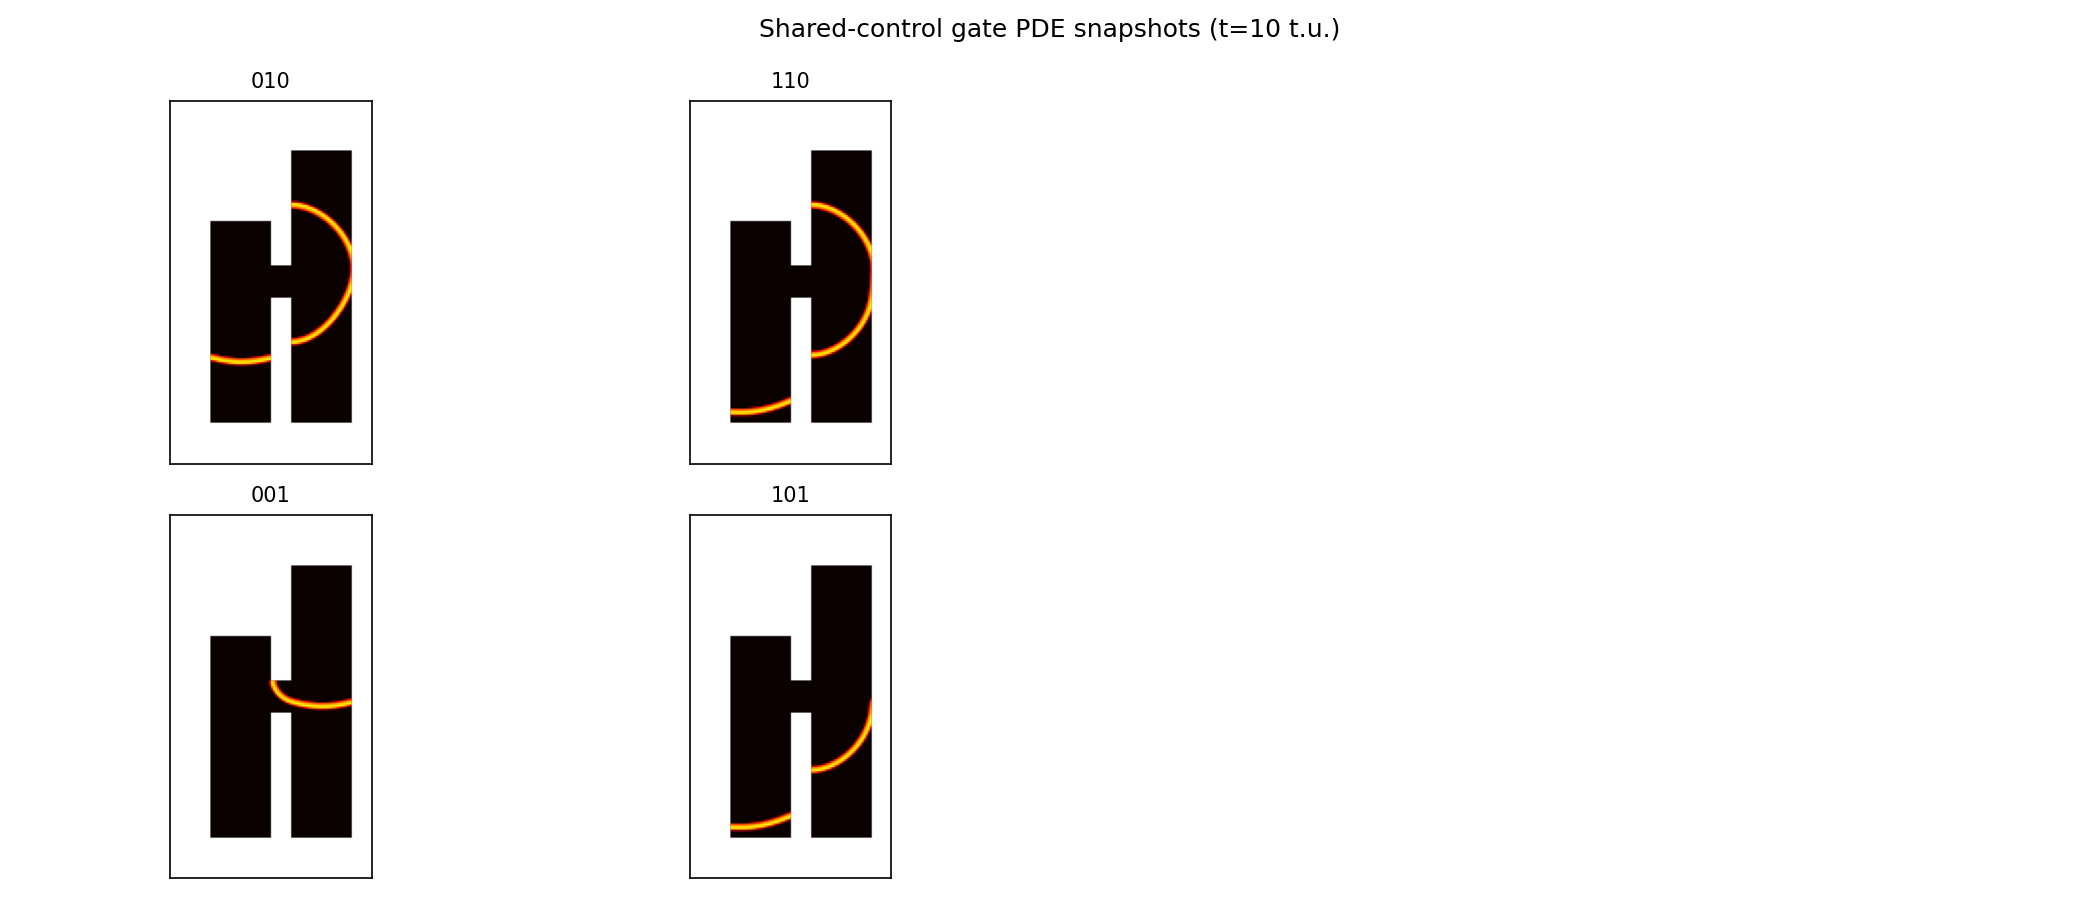
\includegraphics[width=0.95\textwidth]{../Analysis/figures/rd_multi_gate_pde_snapshots.png}}{%
[figure pending]}
\caption{Shared-control multi-junction gate. A single control pulse blocks both data paths, but pattern $011$ produces crosstalk when B1 enters the shared control channel and blocks J2 before B2 arrives.}
\label{fig:res_graph_multi}
\end{figure}

\section{Geometry-Dependent Failure of Collision XOR}
\label{sec:res_xor}

A symmetric Y-junction with a chamber was designed to implement collision XOR: a pulse on either input arm should reach the output, but two coincident pulses should annihilate and leave the output silent.
The graph model predicts this behaviour, but the PDE shows a leak.
\reftab{tab:res_xor} gives the result for a chamber radius $R = 25$ cells.

\begin{table}[htbp]
\centering
\caption{Collision-XOR prediction versus PDE in a chambered Y-junction.}
\label{tab:res_xor}
\small
\begin{tabular}{lcc}
\toprule
Pattern & Graph prediction & PDE (chamber $R = 25$) \\
\midrule
01 / 10 & output fires & output fires \\
11 & no output & output still fires \\
\bottomrule
\end{tabular}
\end{table}

The leak occurs because extended channel fronts collide but the excitation curves around the annihilation point and re-ignites the output stem.
Pattern $11$ still triggers crossings in the output arms, so the chamber geometry does not achieve clean collision XOR.
This confirms that inhibition rules are geometry-dependent: the graph model must be PDE-calibrated per junction shape, not assumed universal.

\begin{figure}[htbp]
\centering
\IfFileExists{../Analysis/figures/rd_spot_xor_protocol.png}{%
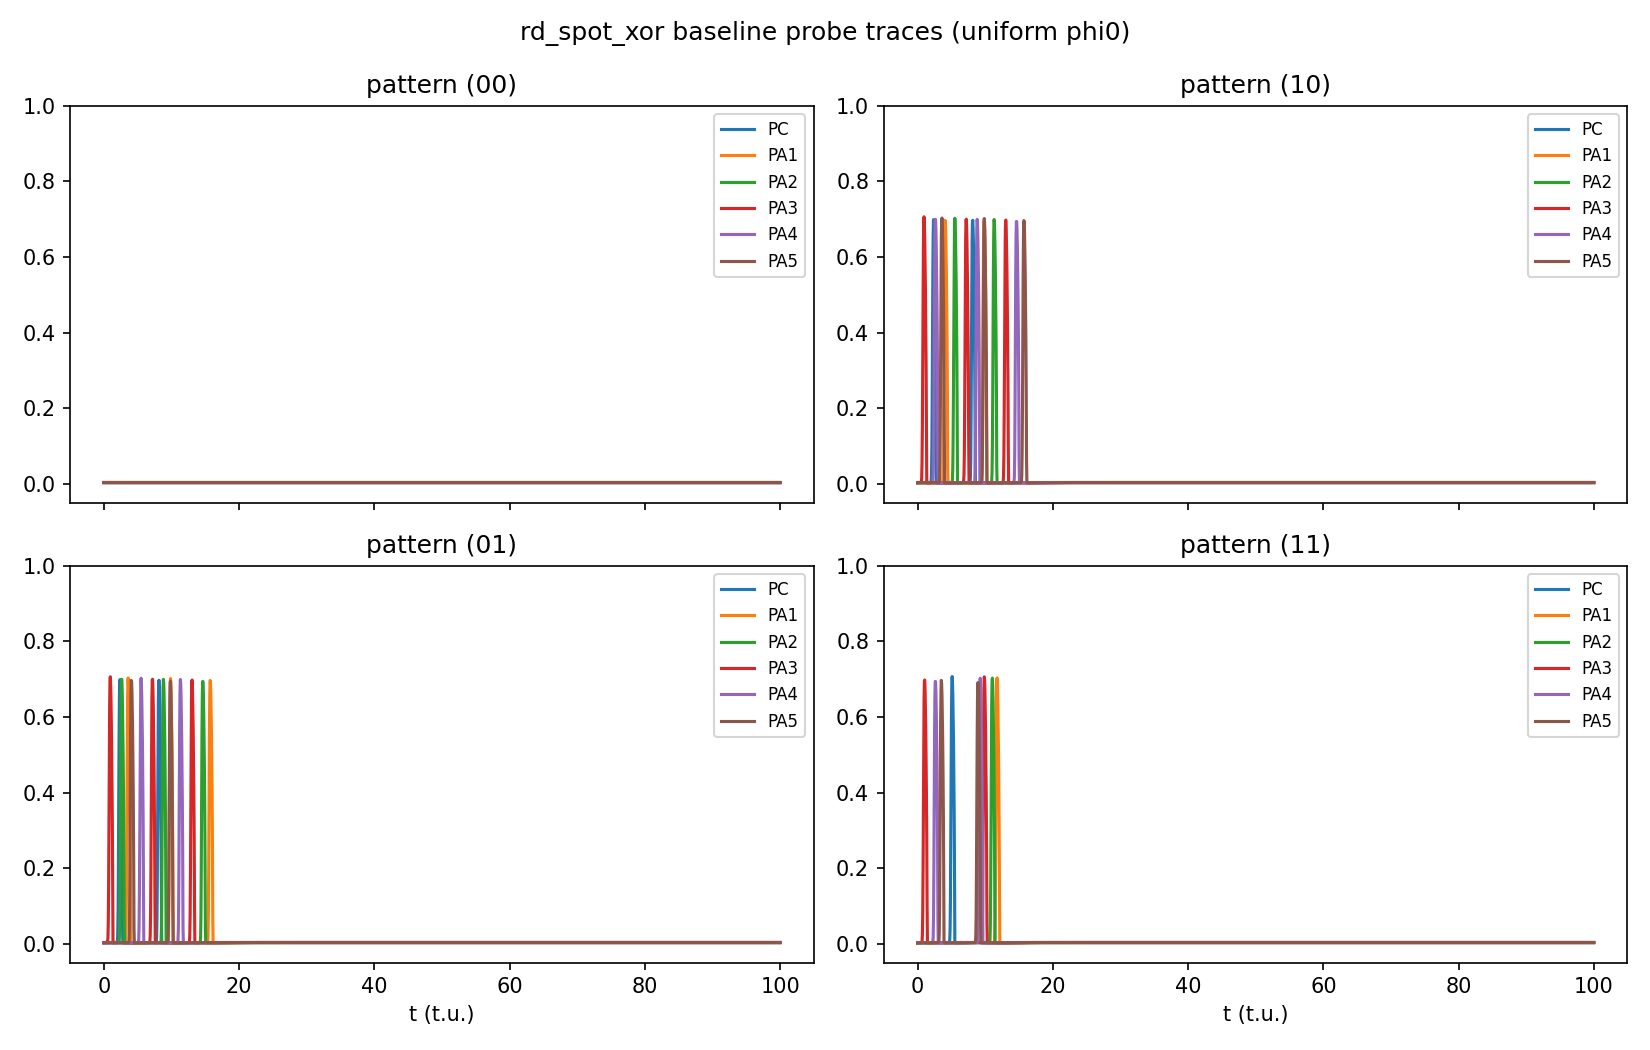
\includegraphics[width=0.95\textwidth]{../Analysis/figures/rd_spot_xor_protocol.png}}{%
[figure pending]}
\caption{Collision-XOR baseline in a chambered Y-junction. Lone input pulses reach the output, but the coincident-pulse case leaks because the collision re-ignites the output stem.}
\label{fig:res_xor}
\end{figure}

\section{Three-Dimensional Inhibition Gate}
\label{sec:res_3d}

The graph simulator is dimensionless, so the same rules apply in three dimensions.
To test whether the 2D operators transfer, a 3D T-junction inhibition gate was simulated in a $64 \times 48 \times 48$ domain.
The original geometry was a `+' intersection in which the vertical B channel had a downward outlet; this allowed B alone to reach the output, giving only a $2.5\times$ separation.
After closing the B outlet arm and scaling the arm lengths, the gate was recognised cleanly.
\reftab{tab:res_3d} gives the corrected 3D truth table.

\begin{table}[htbp]
\centering
\caption{Corrected 3D T-junction inhibition gate.}
\label{tab:res_3d}
\small
\begin{tabular}{ccc}
\toprule
inputs & window peak & comment \\
\midrule
00 & 0.003 & quiet \\
10 (A only) & 0.713 & A passes \\
01 (B only) & 0.042 & suppressed leakage \\
11 (A+B) & 0.042 & suppressed leakage \\
\bottomrule
\end{tabular}
\end{table}

The separation ratio is $16.8\times$ and A alone arrives at the probe at $8.25$ time units.
The 3D channel pulse speed is $6.62$ cells per time unit, close to the 2D value of $6.46$.
This shows that the micro-scale operators do transfer to a thin-slab 3D geometry once the junction shape is controlled.
A full 3D multi-gate network remains future work.

\begin{figure}[htbp]
\centering
\IfFileExists{../Analysis/figures/rd_3d_transfer_logic_snapshots.png}{%
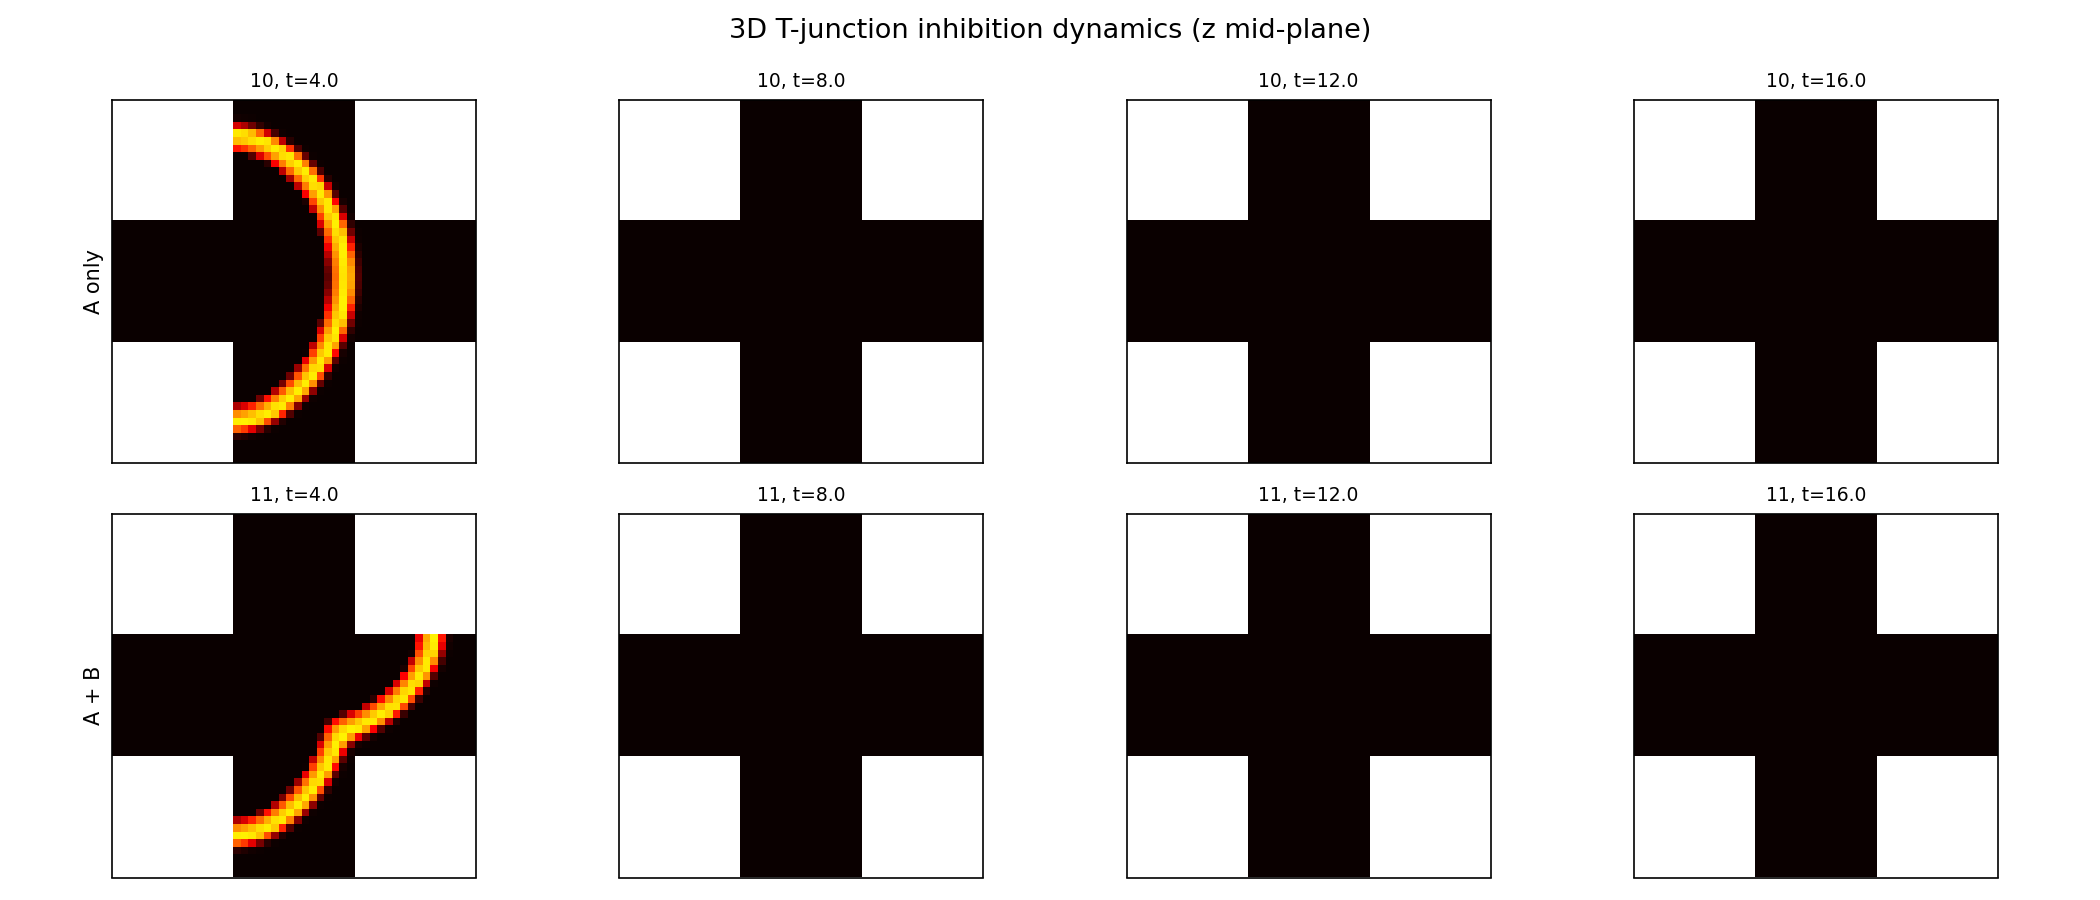
\includegraphics[width=0.95\textwidth]{../Analysis/figures/rd_3d_transfer_logic_snapshots.png}}{%
[figure pending]}
\caption{Three-dimensional T-junction inhibition gate. A alone reaches the output; B alone and A+B are suppressed after closing the B outlet arm and scaling the geometry.}
\label{fig:res_3d}
\end{figure}

\section{One-Way Diode Pilot}
\label{sec:res_diode}

A one-way pulse diode was tested in three forms: an asymmetric wall geometry (gradual taper on one side, abrupt step on the other), a straight channel with an asymmetric $\phi$ barrier, and a hybrid of the two.
\reftab{tab:res_diode} summarises the results.

\begin{table}[htbp]
\centering
\caption{One-way diode pilot results.}
\label{tab:res_diode}
\small
\begin{tabular}{lcccc}
\toprule
mode & forward peak & reverse peak & extinction ratio & diode works? \\
\midrule
geometry & 0.724 & 0.517 & 1.4 & no \\
light & 0.680 & 0.680 & 1.0 & no \\
hybrid & 0.724 & 0.517 & 1.4 & no \\
\bottomrule
\end{tabular}
\end{table}

The asymmetric wall geometry gives only a $1.4\times$ forward-to-reverse ratio, and the reverse pulse still crosses threshold.
The light-only barrier is symmetric because the static $\phi$ field spans both directions equally.
A simple asymmetric taper or static light barrier is therefore insufficient for robust rectification in the present parameter regime.
The diode is left as an open problem; candidate fixes include angled branches, absorbing side chambers, or timed refractory structures.

\begin{figure}[htbp]
\centering
\IfFileExists{../Analysis/figures/rd_diode_pilot_series.png}{%
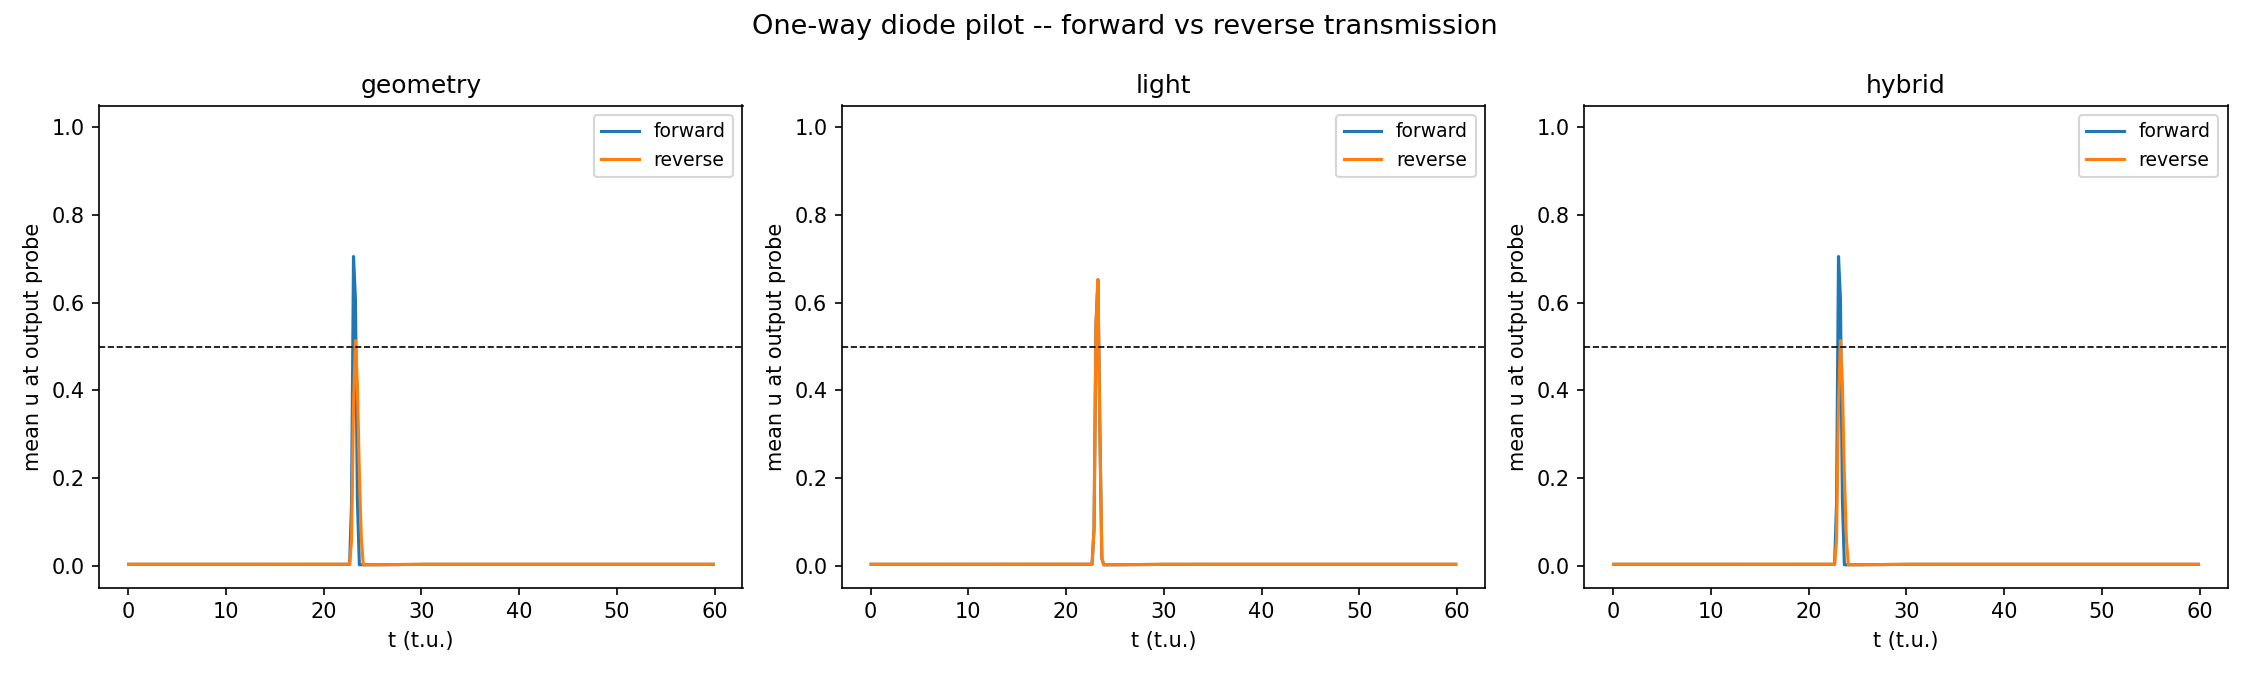
\includegraphics[width=0.95\textwidth]{../Analysis/figures/rd_diode_pilot_series.png}}{%
[figure pending]}
\caption{One-way diode pilot. Asymmetric wall geometry, a static light barrier, and a hybrid of the two all fail to give a robust forward-to-reverse extinction ratio in the present parameter regime.}
\label{fig:res_diode}
\end{figure}

\section{Uncertainty Quantification}
\label{sec:res_uq}

A one-at-a-time sensitivity analysis propagates $\pm 10\%$ uncertainty in the kinetic parameters $\varepsilon$, $f$, $\phi$, and $D_{u}$ to the channel pulse speed and amplitude.
The parameter $f$ dominates the probe peak amplitude, while $\varepsilon$ dominates the pulse speed; $\phi$ and $D_{u}$ have smaller but non-negligible effects.
This gives the characterisation a robustness layer and identifies which parameters must be constrained most tightly in any future experimental realisation.

\begin{figure}[htbp]
\centering
\IfFileExists{../Analysis/figures/pub/pub_sobol_indices.png}{%
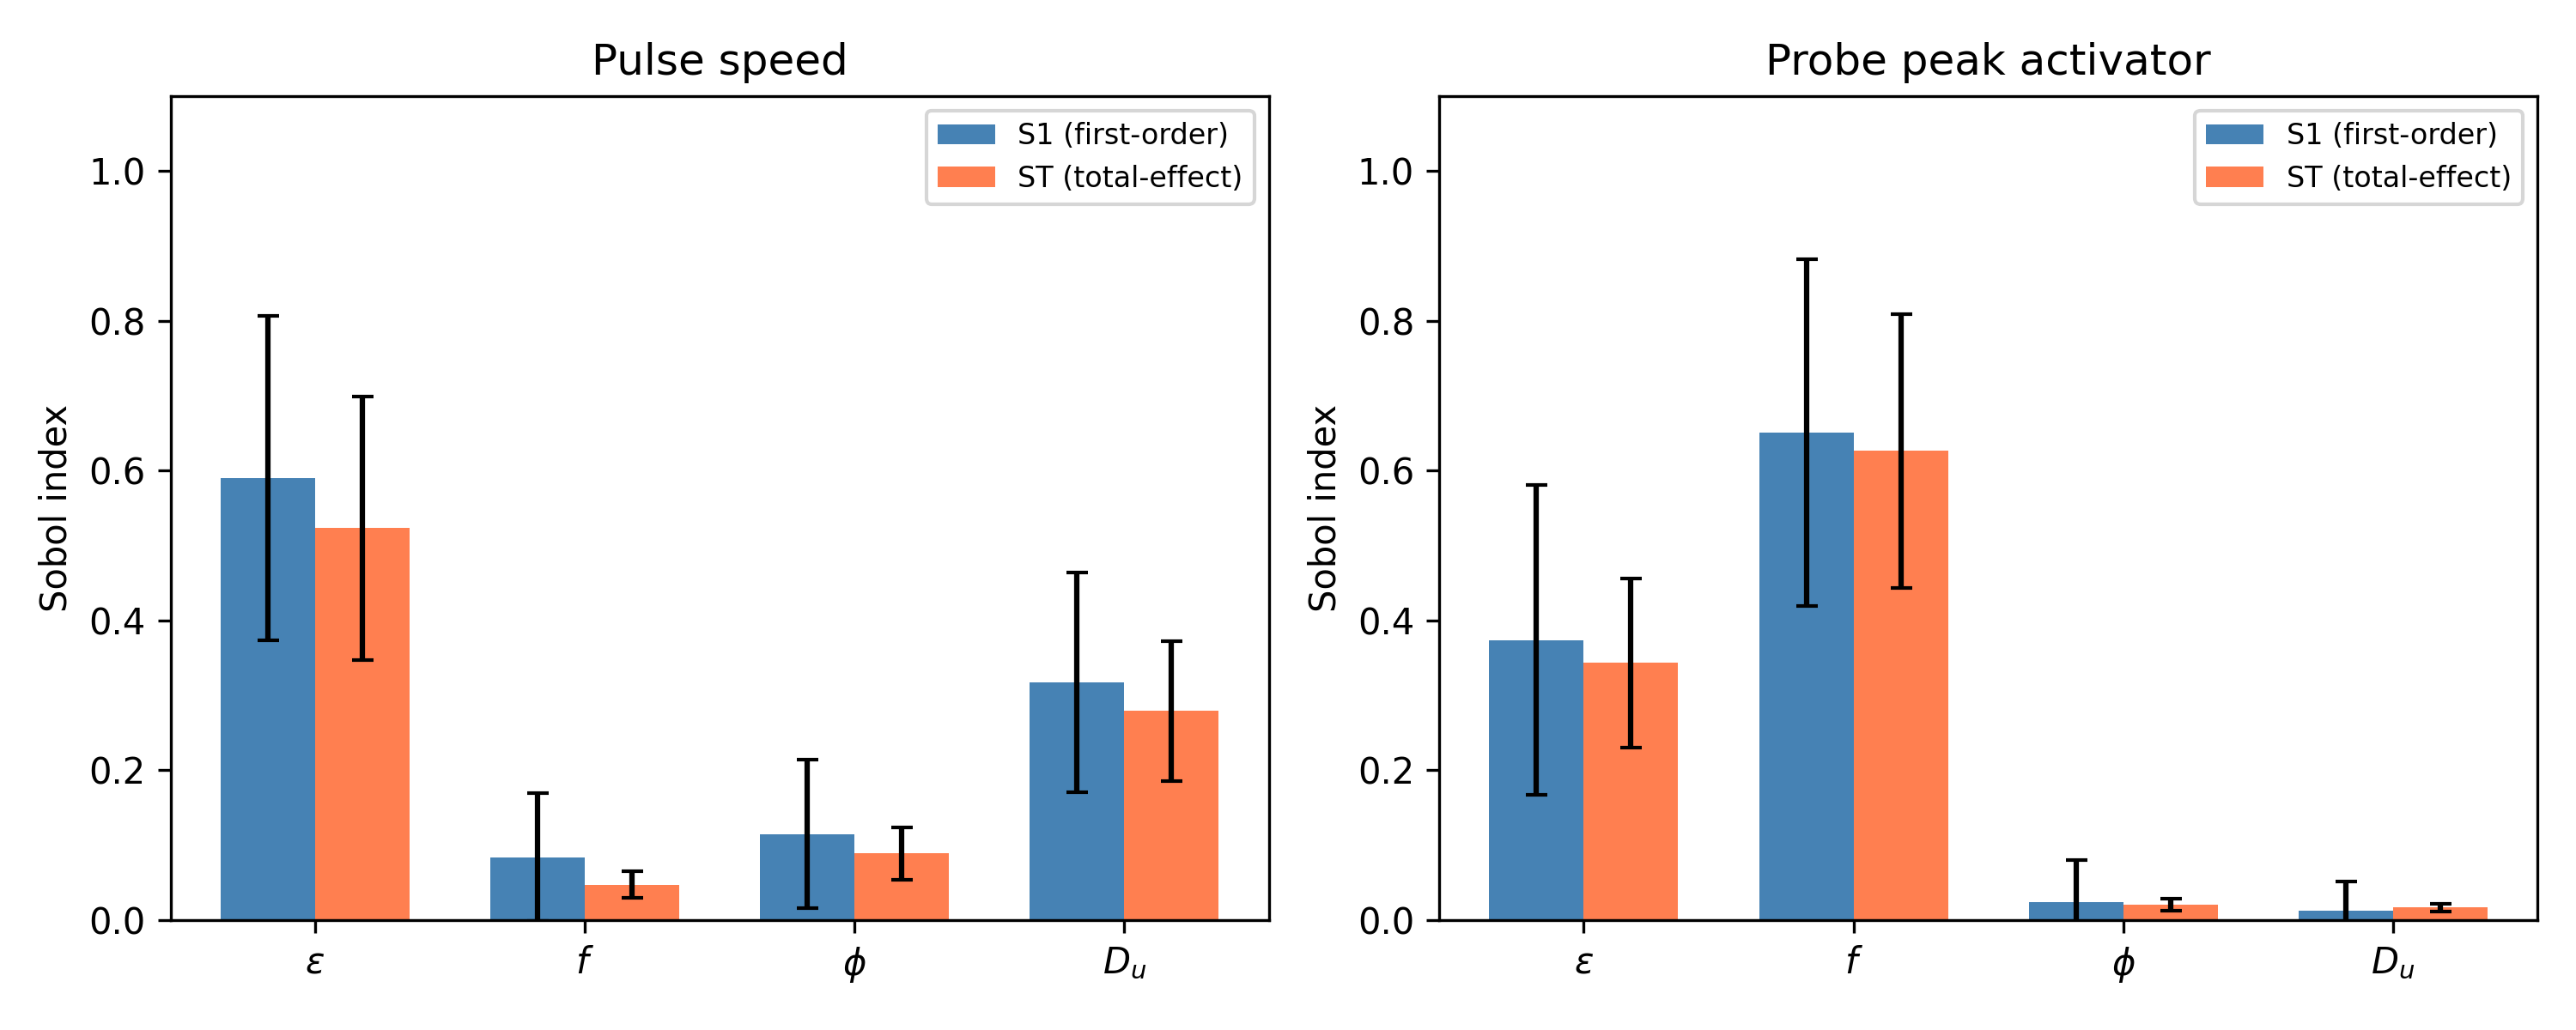
\includegraphics[width=0.9\textwidth]{../Analysis/figures/pub/pub_sobol_indices.png}}{%
[figure pending]}
\caption{One-at-a-time sensitivity of the channel pulse speed and amplitude to $\pm 10\%$ uncertainty in the kinetic parameters. $f$ dominates the amplitude and $\varepsilon$ dominates the speed.}
\label{fig:res_uq}
\end{figure}

\section{Training Attempt}
\label{sec:res_train}

A trainable light-field T-junction directionality task was attempted as a proof of concept.
A $4 \times 4$ bilinear interpolation grid parameterised $\phi(x,y)$ around the junction, and CMA-ES was used to minimise a soft loss that rewards high response at the assigned output and low response at the wrong output.
The task returned a negative result: no trainable improvement over a uniform-phi baseline was found within the optimisation budget.
This marks the practical limit of simple light-field modulation in the present regime and reinforces the characterisation-first framing: the native operators constrain what a training loop can achieve.
